\documentclass{standalone}
\usepackage{tikz}
\usetikzlibrary{patterns, positioning}


\begin{document}
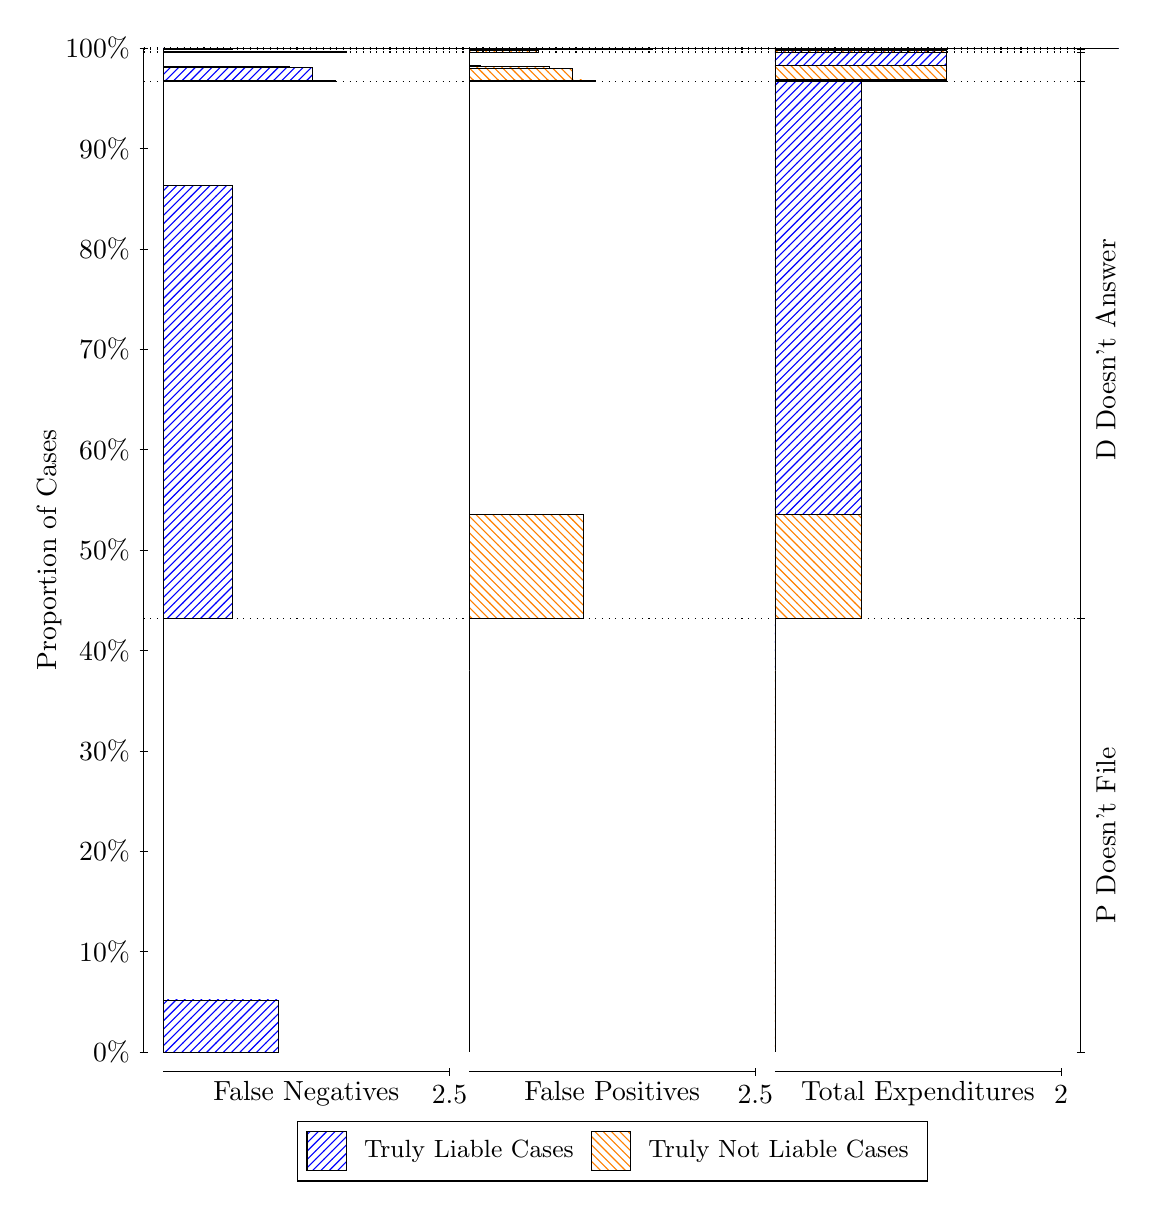
\begin{tikzpicture}
\draw[black, very thin] (1.5,1.75) -- (1.5,14.5);
\node[rotate=90, text=black, anchor=center] at (0.3, 8.125) {Proportion of Cases};
\draw[black, very thin] (1.45,1.75) -- (1.55,1.75);
\node[text=black, anchor=east] at (1.45, 1.75) {0\%};
\draw[black, very thin] (1.45,3.025) -- (1.55,3.025);
\node[text=black, anchor=east] at (1.45, 3.025) {10\%};
\draw[black, very thin] (1.45,4.3) -- (1.55,4.3);
\node[text=black, anchor=east] at (1.45, 4.3) {20\%};
\draw[black, very thin] (1.45,5.575) -- (1.55,5.575);
\node[text=black, anchor=east] at (1.45, 5.575) {30\%};
\draw[black, very thin] (1.45,6.85) -- (1.55,6.85);
\node[text=black, anchor=east] at (1.45, 6.85) {40\%};
\draw[black, very thin] (1.45,8.125) -- (1.55,8.125);
\node[text=black, anchor=east] at (1.45, 8.125) {50\%};
\draw[black, very thin] (1.45,9.4) -- (1.55,9.4);
\node[text=black, anchor=east] at (1.45, 9.4) {60\%};
\draw[black, very thin] (1.45,10.675) -- (1.55,10.675);
\node[text=black, anchor=east] at (1.45, 10.675) {70\%};
\draw[black, very thin] (1.45,11.95) -- (1.55,11.95);
\node[text=black, anchor=east] at (1.45, 11.95) {80\%};
\draw[black, very thin] (1.45,13.225) -- (1.55,13.225);
\node[text=black, anchor=east] at (1.45, 13.225) {90\%};
\draw[black, very thin] (1.45,14.5) -- (1.55,14.5);
\node[text=black, anchor=east] at (1.45, 14.5) {100\%};

\draw[black, very thin] (13.4,1.75) -- (13.4,14.5);
\draw[black, very thin] (13.35,1.75) -- (13.45,1.75);
\node[anchor=west] at (13.35, 1.75) {};
\draw[black, very thin] (13.35,7.2565) -- (13.45,7.2565);
\node[anchor=west] at (13.35, 7.2565) {};
\draw[black, very thin] (13.35,14.078) -- (13.45,14.078);
\node[anchor=west] at (13.35, 14.078) {};
\draw[black, very thin] (13.35,14.45) -- (13.45,14.45);
\node[anchor=west] at (13.35, 14.45) {};
\draw[black, very thin] (13.35,14.48) -- (13.45,14.48);
\node[anchor=west] at (13.35, 14.48) {};
\draw[black, very thin] (13.35,14.5) -- (13.45,14.5);
\node[anchor=west] at (13.35, 14.5) {};
\draw[black, very thin] (13.35,14.5) -- (13.45,14.5);
\node[anchor=west] at (13.35, 14.5) {};
\draw[black, very thin] (13.35,14.5) -- (13.45,14.5);
\node[anchor=west] at (13.35, 14.5) {};

\draw[black, very thin, pattern color=blue, pattern=north east lines] (1.75,1.75) rectangle (3.2033,2.4126);
\draw[black, very thin, pattern color=orange, pattern=north west lines] (1.75,2.4126) rectangle (1.75,7.2565);
\draw[black, very thin, pattern color=blue, pattern=north east lines] (1.75,7.2565) rectangle (2.622,12.759);
\draw[black, very thin, pattern color=orange, pattern=north west lines] (1.75,12.759) rectangle (1.75,14.078);
\draw[black, very thin, pattern color=blue, pattern=north east lines] (1.75,14.078) rectangle (3.93,14.09);
\draw[black, very thin, pattern color=blue, pattern=north east lines] (1.75,14.09) rectangle (3.7847,14.091);
\draw[black, very thin, pattern color=blue, pattern=north east lines] (1.75,14.091) rectangle (3.6393,14.25);
\draw[black, very thin, pattern color=blue, pattern=north east lines] (1.75,14.25) rectangle (3.494,14.252);
\draw[black, very thin, pattern color=blue, pattern=north east lines] (1.75,14.252) rectangle (3.3487,14.264);
\draw[black, very thin, pattern color=orange, pattern=north west lines] (1.75,14.264) rectangle (1.75,14.45);
\draw[black, very thin, pattern color=blue, pattern=north east lines] (1.75,14.45) rectangle (4.0753,14.461);
\draw[black, very thin, pattern color=orange, pattern=north west lines] (1.75,14.461) rectangle (1.75,14.48);
\draw[black, very thin, pattern color=blue, pattern=north east lines] (1.75,14.48) rectangle (2.622,14.493);
\draw[black, very thin, pattern color=orange, pattern=north west lines] (1.75,14.493) rectangle (1.75,14.5);
\draw[black, very thin, pattern color=blue, pattern=north east lines] (1.75,14.5) rectangle (7.5633,14.5);
\draw[black, very thin, pattern color=orange, pattern=north west lines] (1.75,14.5) rectangle (1.75,14.5);
\draw[black, very thin, pattern color=orange, pattern=north west lines] (1.75,14.5) rectangle (1.75,14.5);
\draw[black, very thin, pattern color=blue, pattern=north east lines] (1.75,14.5) rectangle (1.75,14.5);
\draw[black, very thin, pattern color=orange, pattern=north west lines] (5.6333,1.75) rectangle (5.6333,6.5939);
\draw[black, very thin, pattern color=blue, pattern=north east lines] (5.6333,6.5939) rectangle (5.6333,7.2565);
\draw[black, very thin, pattern color=orange, pattern=north west lines] (5.6333,7.2565) rectangle (7.0867,8.5755);
\draw[black, very thin, pattern color=blue, pattern=north east lines] (5.6333,8.5755) rectangle (5.6333,14.078);
\draw[black, very thin, pattern color=orange, pattern=north west lines] (5.6333,14.078) rectangle (7.232,14.092);
\draw[black, very thin, pattern color=orange, pattern=north west lines] (5.6333,14.092) rectangle (7.0867,14.094);
\draw[black, very thin, pattern color=orange, pattern=north west lines] (5.6333,14.094) rectangle (6.9413,14.242);
\draw[black, very thin, pattern color=orange, pattern=north west lines] (5.6333,14.242) rectangle (6.796,14.242);
\draw[black, very thin, pattern color=orange, pattern=north west lines] (5.6333,14.242) rectangle (6.6507,14.265);
\draw[black, very thin, pattern color=blue, pattern=north east lines] (5.6333,14.265) rectangle (5.7787,14.277);
\draw[black, very thin, pattern color=blue, pattern=north east lines] (5.6333,14.277) rectangle (5.6333,14.45);
\draw[black, very thin, pattern color=orange, pattern=north west lines] (5.6333,14.45) rectangle (6.5053,14.469);
\draw[black, very thin, pattern color=blue, pattern=north east lines] (5.6333,14.469) rectangle (5.6333,14.48);
\draw[black, very thin, pattern color=orange, pattern=north west lines] (5.6333,14.48) rectangle (7.9587,14.487);
\draw[black, very thin, pattern color=blue, pattern=north east lines] (5.6333,14.487) rectangle (6.5053,14.5);
\draw[black, very thin, pattern color=orange, pattern=north west lines] (5.6333,14.5) rectangle (5.6333,14.5);
\draw[black, very thin, pattern color=blue, pattern=north east lines] (5.6333,14.5) rectangle (5.6333,14.5);
\draw[black, very thin, pattern color=orange, pattern=north west lines] (5.6333,14.5) rectangle (11.447,14.5);
\draw[black, very thin, pattern color=blue, pattern=north east lines] (5.6333,14.5) rectangle (9.9933,14.5);
\draw[black, very thin, pattern color=orange, pattern=north west lines] (9.5167,1.75) rectangle (9.5167,6.5939);
\draw[black, very thin, pattern color=blue, pattern=north east lines] (9.5167,6.5939) rectangle (9.5167,7.2565);
\draw[black, very thin, pattern color=orange, pattern=north west lines] (9.5167,7.2565) rectangle (10.607,8.5755);
\draw[black, very thin, pattern color=blue, pattern=north east lines] (9.5167,8.5755) rectangle (10.607,14.078);
\draw[black, very thin, pattern color=orange, pattern=north west lines] (9.5167,14.078) rectangle (11.697,14.092);
\draw[black, very thin, pattern color=blue, pattern=north east lines] (9.5167,14.092) rectangle (11.697,14.105);
\draw[black, very thin, pattern color=orange, pattern=north west lines] (9.5167,14.105) rectangle (11.697,14.277);
\draw[black, very thin, pattern color=blue, pattern=north east lines] (9.5167,14.277) rectangle (11.697,14.45);
\draw[black, very thin, pattern color=orange, pattern=north west lines] (9.5167,14.45) rectangle (11.697,14.469);
\draw[black, very thin, pattern color=blue, pattern=north east lines] (9.5167,14.469) rectangle (11.697,14.48);
\draw[black, very thin, pattern color=orange, pattern=north west lines] (9.5167,14.48) rectangle (11.697,14.487);
\draw[black, very thin, pattern color=blue, pattern=north east lines] (9.5167,14.487) rectangle (11.697,14.5);
\draw[black, very thin, pattern color=orange, pattern=north west lines] (9.5167,14.5) rectangle (13.877,14.5);
\draw[black, very thin, pattern color=blue, pattern=north east lines] (9.5167,14.5) rectangle (13.877,14.5);
\draw[black, very thin, pattern color=orange, pattern=north west lines] (9.5167,14.5) rectangle (13.877,14.5);
\draw[black, very thin, pattern color=blue, pattern=north east lines] (9.5167,14.5) rectangle (13.877,14.5);
\draw[black, dotted] (1.5,7.2565) -- (13.4,7.2565);
\draw[black, dotted] (1.5,14.078) -- (13.4,14.078);
\draw[black, dotted] (1.5,14.45) -- (13.4,14.45);
\draw[black, dotted] (1.5,14.48) -- (13.4,14.48);
\draw[black, dotted] (1.5,14.5) -- (13.4,14.5);
\draw[black, dotted] (1.5,14.5) -- (13.4,14.5);
\draw[black, very thin] (1.75,1.5) -- (5.3833,1.5);
\node[text=black, anchor=north] at (3.5667, 1.5) {False Negatives};
\draw[black, very thin] (5.3833,1.45) -- (5.3833,1.55);
\node[text=black, anchor=north] at (5.3833, 1.45) {2.5};

\draw[black, very thin] (5.6333,1.5) -- (9.2667,1.5);
\node[text=black, anchor=north] at (7.45, 1.5) {False Positives};
\draw[black, very thin] (9.2667,1.45) -- (9.2667,1.55);
\node[text=black, anchor=north] at (9.2667, 1.45) {2.5};

\draw[black, very thin] (9.5167,1.5) -- (13.15,1.5);
\node[text=black, anchor=north] at (11.333, 1.5) {Total Expenditures};
\draw[black, very thin] (13.15,1.45) -- (13.15,1.55);
\node[text=black, anchor=north] at (13.15, 1.45) {2};

\node[text=black, centered, rotate=90] at (13.72, 4.5033) {P Doesn't File};
\node[text=black, centered, rotate=90] at (13.72, 10.667) {D Doesn't Answer};






\draw (7.449999999999999,1.5) node[draw=none] (baseCoordinate) {};
\begin{scope}[align=center]
        \matrix[scale=0.5, draw=black, below=0.5cm of baseCoordinate, nodes={draw}, column sep=0.1cm]{
            \node[rectangle, draw, minimum width=0.5cm, minimum height=0.5cm, pattern color=blue, pattern=north east lines] {}; &
            \node[draw=none, font=\small, text=black] (B) {Truly Liable Cases}; &
            \node[rectangle, draw, minimum width=0.5cm, minimum height=0.5cm, pattern color=orange, pattern=north west lines] {}; &
            \node[draw=none, font=\small, text=black] (B) {Truly Not Liable Cases}; \\
            };
\end{scope}

\end{tikzpicture}
\end{document}